\documentclass[12pt]{article}

\usepackage{amsmath}
\usepackage{graphicx}
\usepackage{float}

\begin{document}

\title{Exercise: \LaTeX}
\author{Wikipedia \& Asger Gardner}

\maketitle

\section*{i)}

The exponential function is a mathematical function denoted by $f(x)=\text{exp}(x)$ or $e^{x}$ (where the argument x is written as an exponent). It can be defined in several equivalent ways. Its ubiquitous occurrence in pure and applied mathematics led mathematician Walter Rudin to opine that the exponential function is "the most important function in mathematics". 

\section*{ii)}

In this short report, the continued-fraction representation \eqref{eq:cf_ex} of the exponential function is considered.  

\begin{equation} \label{eq:cf_ex}
	e^x = 1 + \cfrac{x}{1 - \cfrac{x}{x + 2 - \cfrac{2x}{x + 3 - \cfrac{3x}{x + 4 - \ddots}}}}
\end{equation}

The continued fraction is obtained by an Euler identity connecting infinite series with infinite continued fractions. Since the exponential function can be formally defined as an infinite power series, an infinite continued fraction would be an equivalent definition. However, computing an infinite series would require an infinite amount of computations, and would thus run forever on a computer. In order to prevent this unfortunate circumstance, the approximation is only ran until the 10th term in this case.

\section*{iii)}

In order to test whether the 10th term continued fraction approximation \eqref{eq:cf_ex} works, it is compared to the C-sharp system definition, System.Math.Exp. This comparison is shown in figure \ref{fig:ex}. From this figure, it is gathered that \eqref{eq:cf_ex} is a sufficient approximation. 

\begin{figure}[H] \label{fig:ex}
	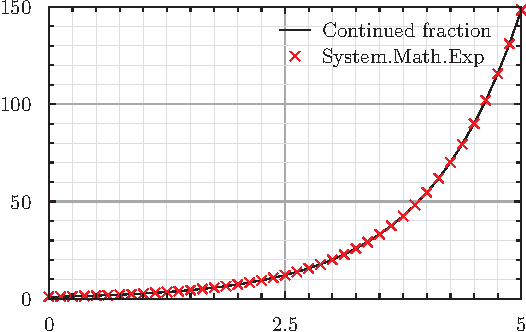
\includegraphics[width=\linewidth]{explot.pdf}
\end{figure}

\end{document}
